\section{جهت ۲: \lr{low-rank adaptation of the text encoder}}
\label{sec:d2}
\begin{keybox}[شاخه: \branch{direction2-ordinal-text-lora}]
درجه‌ها با ۲۵ توصیف بالینی واقعی بیان می‌شوند و خود \lr{text encoder} با \lr{LoRA} برای درجه‌بندی \lr{DR} تنظیم می‌شود. ترتیب روی خروجی \lr{text encoder} اعمال می‌شود، پس \lr{encoder} تطبیق‌یافته، و نه فقط پنج بردار، ترتیب درجه‌ها را می‌آموزد.
\end{keybox}

شکل~\ref{fig:wf-d2} گردش کار کامل جهت ۲ را نشان می‌دهد: ۲۵ توصیف بالینی از \lr{text encoder} تطبیق‌یافته با \lr{LoRA} می‌گذرند و \lr{constraint}های ترتیبی روی خروجی آن اعمال می‌شوند. \lr{protocol} آزمایش‌ها در شکل~\ref{fig:proto-d2} آمده است.

\begin{landscape}
\begin{figure}[p]
\centering
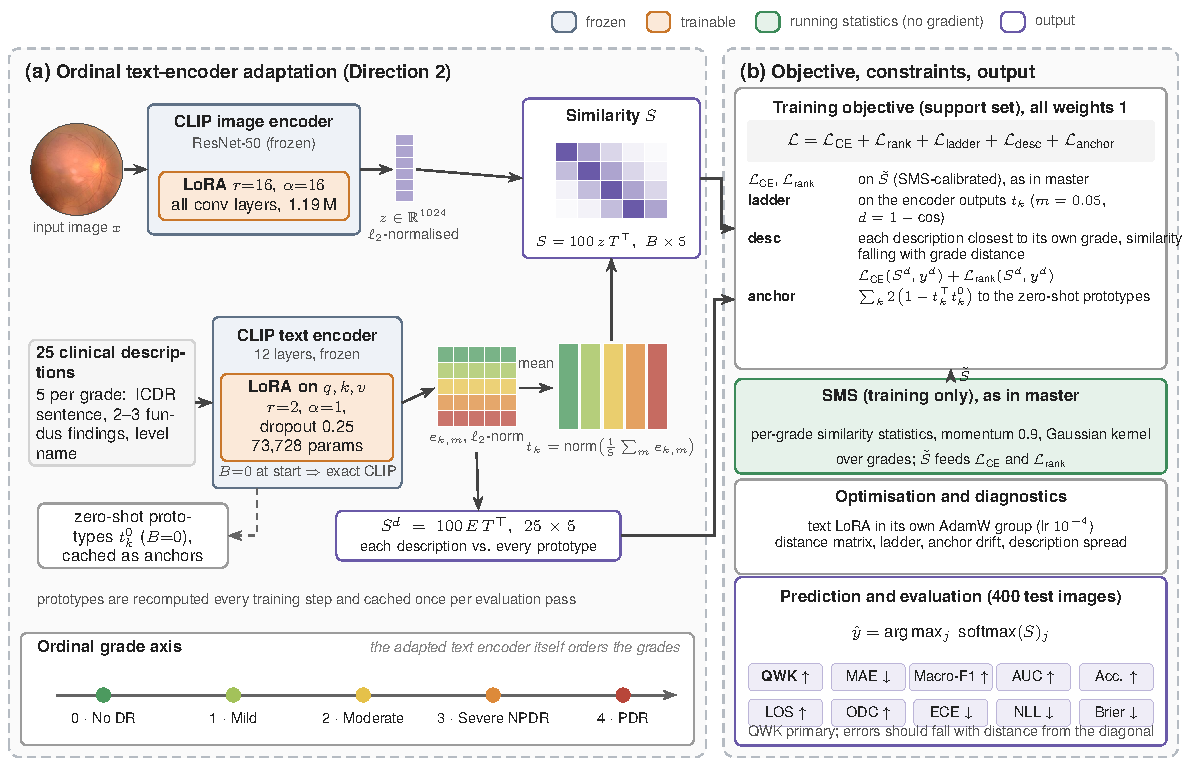
\includegraphics[width=\linewidth]{workflow_d2}
\caption{گردش کار کامل جهت ۲: توصیف‌های بالینی، \lr{LoRA} روی $q$، $k$ و $v$ \lr{text encoder}، \lr{prototype}ها میانگین، \lr{similarity matrix} توصیف‌ها $S^d$ و \lr{loss function} با \lr{constraint}های \lr{ladder}، \lr{description ordering} و \lr{anchor}.}
\label{fig:wf-d2}
\end{figure}
\end{landscape}

% ------------------------------------------------------------------
\subsection{انگیزه و شکاف پژوهشی}
مدل پایه \lr{prompt} را می‌آموزد و جهت ۱ \lr{grade vector}ها را؛ در هر دو، دانش زبانی فقط در نقطهٔ شروع حضور دارد. جهت ۲ برعکس عمل می‌کند: درجه‌ها با زبان بالینی واقعی توصیف می‌شوند و این بار خود \lr{text encoder}، با \lr{low-rank adaptation}، برای درجه‌بندی \lr{DR} تنظیم می‌شود. ایده از \lr{CLIP-LoRA} \cite{cliplora} گرفته شده که \lr{LoRA} را روی هر دو \lr{encoder} اعمال می‌کند، اما آن روش برای کلاس‌های بدون ترتیب طراحی شده است. نوآوری جهت ۲ این است که ترتیب روی خروجی \lr{text encoder} اعمال می‌شود. یک پیامد عملی هم دارد: توصیف تازه‌ای از یک درجه را می‌توان بدون آموزش دوباره کدگذاری کرد.

\begin{figure}[H]
\begin{diagram}
  \node[frozen=3.4cm] (a) {\textbf{Master / Dir.~1}\\ language knowledge only at init};
  \node[frozen=3.4cm,left=12mm of a] (b) {\textbf{CLIP-LoRA}\\ LoRA on both encoders, no ordering};
  \node[train=6.4cm,below=14mm of $(a)!0.5!(b)$] (c) {\textbf{Dir.~2:} clinical descriptions + text LoRA + ordinal constraint on text output};
  \node[datan=6.4cm,below=of c] (d) {Benefit: new description encoded without retraining};
  \draw[arr] (a) -- (c); \draw[arr] (b) -- (c); \draw[arr] (c)--(d);
\end{diagram}
\caption{شکاف پژوهشی جهت ۲.}
\label{fig:d2-gap}
\end{figure}

% ------------------------------------------------------------------
\subsection{تفاوت با مدل پایه}
\begin{table}[H]
\caption{آنچه در جهت ۲ تغییر می‌کند}
\label{tab:d2-diff}
\centering\small
\begin{tabularx}{\textwidth}{@{}p{3.6cm} X X@{}}
\toprule
\textbf{جزء} & \textbf{مدل پایه} & \textbf{جهت ۲}\\
\midrule
ورودی \lr{text branch} & توکن‌های \lr{learnable} & ۲۵ توصیف بالینی ثابت (۵ برای هر درجه)\\
\lr{text encoder} & \lr{frozen} & \lr{frozen} + \lr{LoRA} روی \lr{q}، \lr{k} و \lr{v} در هر ۱۲ لایه\\
\lr{prototype} درجه & خروجی یک \lr{prompt} & میانگین نرمال‌شدهٔ ۵ توصیف\\
\lr{constraint} ترتیبی روی نمایش & \lr{interpolation} توکن‌ها & \lr{ladder}، \lr{description ordering}، \lr{anchor}\\
\lr{image branch}، داده، \lr{SMS}، \lr{loss} رتبه، \lr{metric}ها، آموزش & \multicolumn{2}{l}{یکسان با بخش~\ref{sec:master}}\\
\bottomrule
\end{tabularx}
\end{table}

% ------------------------------------------------------------------
\subsection{معماری}
\begin{figure}[H]
\begin{diagram}
  \node[datan=3.6cm] (d) {25 clinical descriptions\\ 5 per grade};
  \node[train=3.6cm,below=of d] (te) {CLIP text encoder\\ frozen + LoRA on q, k, v};
  \node[box=3.6cm,below=of te] (e) {$e_{k,m}$: normalised description vector};
  \node[box=3.6cm,below=of e] (m) {Mean per grade + normalise: $t_0\dots t_4$};
  \node[datan=2.6cm,left=40mm of d] (x) {Image};
  \node[train=3cm,below=of x] (v) {CLIP RN50 + LoRA};
  \node[box=3.4cm,below=34mm of v] (s) {$s = 100\cdot z\,t^{\top}$};
  \node[box=2.6cm,below=of s] (sms) {SMS};
  \node[lossn=3.2cm,below=of sms] (l1) {CE + rank-aware loss};
  \node[lossn=2.4cm,below left=12mm and -14mm of m] (l2) {Ladder on $t$};
  \node[lossn=2.4cm,right=4mm of l2] (l4) {Anchor to zero-shot prototypes};
  \node[lossn=2.4cm,right=4mm of l4] (l3) {Desc.~ordering};
  \draw[arr] (d)--(te); \draw[arr] (te)--(e); \draw[arr] (e)--(m);
  \draw[arr] (x)--(v); \draw[arr] (v)--node[elabel,right]{$z$}(s); \draw[arr] (m) -- (s);
  \draw[arr] (s)--(sms); \draw[arr] (sms)--(l1);
  \draw[arr] (m)--(l2); \draw[arr] (m) -- (l4);
  \draw[arr] (e.east) -| (l3.north);
  \begin{scope}[on background layer]\node[group,fit=(d)(te)(e)(m)] (gt) {};\end{scope}
  \node[grouplabel,anchor=south] at (gt.north) {Text branch};
\end{diagram}
\archlegend
\caption{معماری جهت ۲. \lr{LoRA} متن و \lr{LoRA} تصویر هم‌زمان آموخته می‌شوند.}
\label{fig:d2-arch}
\end{figure}

% ------------------------------------------------------------------
\subsection{توصیف‌های بالینی}
برای هر درجه پنج توصیف به زبان انگلیسی نوشته شده است: جملهٔ بالینی جهت ۱، دو یا سه جمله دربارهٔ یافته‌های معمول فوندوس در آن درجه (میکروآنوریسم، خونریزی نقطه‌ای و لکه‌ای، اگزودای سخت، لکهٔ پنبه‌ای، تسبیحی شدن وریدها، ناهنجاری‌های ریزرگی درون شبکیه، نئوواسکولاریزاسیون) و یک جمله که سطح \lr{ICDR} را نام می‌برد. همهٔ توصیف‌ها در محدودهٔ ۷۷ توکن \lr{CLIP} جا می‌شوند. میانگین‌گیری چند توصیف (\lr{CuPL} \cite{cupl}) وابستگی \lr{prototype} به جمله‌بندی یک جملهٔ خاص را کم می‌کند.

\begin{table}[H]
\caption{نمونهٔ توصیف‌های درجهٔ ۳ (شدید غیرتکثیری)}
\label{tab:d2-desc}
\centering\small
\begin{tabularx}{\textwidth}{@{}c X@{}}
\toprule
\textbf{\#} & \textbf{توصیف}\\
\midrule
۱ & \ensent{A fundus photograph showing severe non-proliferative diabetic retinopathy, with extensive intraretinal hemorrhages in four quadrants, venous beading, or intraretinal microvascular abnormalities.}\\
۲ & \ensent{A retina with many intraretinal hemorrhages in all four quadrants and definite venous beading.}\\
۳ & \ensent{A color fundus image with intraretinal microvascular abnormalities and widespread hemorrhages but no new vessels.}\\
۴ & \ensent{Severe diabetic retinopathy meeting the 4-2-1 rule, without neovascularization.}\\
۵ & \ensent{Fundus photography graded as ICDR level 3, severe non-proliferative retinopathy.}\\
\bottomrule
\end{tabularx}
\end{table}

\begin{figure}[H]
\begin{diagram}
  \node[datan=3.6cm] (s1) {ICDR clinical sentence (Dir.~1)};
  \node[datan=3.6cm,right=4mm of s1] (s2) {2--3 fundus-finding sentences};
  \node[datan=3.6cm,right=4mm of s2] (s3) {ICDR level-name sentence};
  \node[box=6cm,below=12mm of s2] (e) {Encode each sentence and normalise: $e_{k,1}\dots e_{k,5}$};
  \node[train=6cm,below=of e] (t) {$t_k$ = normalised mean, Eq.~\ref{eq:d2-proto}};
  \draw[arr] (s1) |- (e.west); \draw[arr] (s2)--(e); \draw[arr] (s3) |- (e.east); \draw[arr] (e)--(t);
\end{diagram}
\caption{ساختن \lr{prototype} هر درجه از پنج توصیف.}
\label{fig:d2-desc}
\end{figure}

% ------------------------------------------------------------------
\subsection{\lr{low-rank adaptation of the text encoder}}
لایه‌های توجه \lr{text encoder} \lr{CLIP}، ماتریس‌های \lr{query}، کلید و مقدار را در یک ماتریس بسته‌بندی‌شده نگه می‌دارند و ابزارهای رایج \lr{LoRA} نمی‌توانند هر کدام را جداگانه هدف بگیرند. به همین دلیل، مطابق \lr{CLIP-LoRA}، هر \lr{attention block} با \lr{block}ی جایگزین می‌شود که وزن‌های \lr{frozen} را نگه می‌دارد و به‌روزرسانی کم‌رتبه را با \lr{dropout} روی ورودی می‌افزاید:
\begin{equation}
h_{\star} = W_{\star}\, x + \frac{\alpha}{r}\, B_{\star} A_{\star}\, \mathrm{dropout}(x), \qquad \star \in \{q, k, v\}
\label{eq:textlora}
\end{equation}
تنظیمات پیش‌فرض \lr{CLIP-LoRA} به کار می‌رود: $r=2$، $\alpha=1$ (ضریب \LRE{۰٫۵}) و \lr{dropout} \LRE{۰٫۲۵}، روی هر ۱۲ لایه. ماتریس $B$ با صفر آغاز می‌شود و آزمون نشان داده است که در این حالت خروجی \lr{encoder} دقیقاً با \lr{CLIP} اصلی برابر است. تعداد \lr{parameter}های \lr{LoRA} متن $12 \times 3 \times 2 \times 2 \times 512$ = \LRE{۷۳٬۷۲۸} است.
\begin{equation}
e_{k,m} = \frac{g_{\theta}(s_{k,m})}{\lVert g_{\theta}(s_{k,m}) \rVert}, \qquad t_k = \frac{\frac{1}{M} \sum_{m=1}^{M} e_{k,m}}{\big\lVert \frac{1}{M} \sum_{m} e_{k,m} \big\rVert}, \qquad M = 5
\label{eq:d2-proto}
\end{equation}
در ارزیابی، \lr{prototype}ها در طول یک دور ارزیابی تغییر نمی‌کنند و یک بار محاسبه می‌شوند. \lr{prototype}ها \lr{zero-shot} (با $B=0$) به‌عنوان \lr{anchor} $t^{0}_k$ نگه داشته می‌شوند.

\begin{figure}[H]
\begin{diagram}
  \node[datan=1.8cm] (x) {$x$ (tokens)};
  \node[frozen=3.6cm,right=12mm of x,yshift=12mm] (w) {$W_q,W_k,W_v$ frozen\\ (packed matrix)};
  \node[train=3.6cm,right=12mm of x,yshift=-12mm] (l) {dropout 0.25 $\rightarrow$ $A\ (r{=}2)$ $\rightarrow$ $B$ $\rightarrow$ $\times 0.5$};
  \node[circle,draw=navy,thick,inner sep=1pt,right=10mm of $(w.east)!0.5!(l.east)$] (p) {$+$};
  \node[frozen=2.8cm,right=8mm of p] (att) {Multi-head attention \& rest of layer};
  \draw[arr] (x) |- (w); \draw[arr] (x) |- (l); \draw[arr] (w) -| (p); \draw[arr] (l) -| (p); \draw[arr] (p)--(att);
\end{diagram}
\caption{\lr{attention block} بازنویسی‌شده با \lr{LoRA} روی \lr{q}، \lr{k} و \lr{v} (رابطهٔ~\ref{eq:textlora}).}
\label{fig:d2-lora}
\end{figure}

% ------------------------------------------------------------------
\subsection{\lr{constraint}های ترتیبی روی خروجی متن}
\paragraph{\lr{ladder} روی \lr{prototype}ها.} همان رابطهٔ~\ref{eq:ladder} جهت ۱، این بار روی $t_k$ که خروجی \lr{encoder} است.

\paragraph{\lr{description ordering}.} هر توصیف باید بیشترین \lr{similarity} را با درجهٔ خودش داشته باشد و \lr{similarity} آن با درجه‌های دیگر با فاصله کاهش یابد. \lr{similarity matrix} $25\times5$ توصیف‌ها و \lr{prototype}ها ساخته می‌شود و همان زوج \lr{loss} \lr{image branch} روی آن اعمال می‌شود:
\begin{equation}
S^{d}_{(k,m), j} = 100 \cdot e_{k,m}^{\top} t_j, \qquad \mathcal{L}_{\mathrm{desc}} = \mathcal{L}_{\mathrm{CE}}(S^{d}, y^{d}) + \mathcal{L}_{\mathrm{rank}}(S^{d}, y^{d})
\label{eq:desc}
\end{equation}
این \lr{constraint} ابر توصیف‌های هر درجه را از درجه‌های دیگر جدا و در امتداد محور درجه مرتب نگه می‌دارد. اگر \lr{encoder} برای کم کردن \lr{loss} تصویر، توصیف‌های دو درجهٔ همسایه را روی هم بیندازد، این \lr{constraint} جلوی آن را می‌گیرد.

\paragraph{\lr{anchor}.} رابطهٔ~\ref{eq:anchor} با $t^{0}_k$ \lr{zero-shot}، تا \lr{encoder} در \lr{regime} بسیار \lr{few-shot} از دانش اولیه دور نشود.

\begin{equation}
\mathcal{L} = \mathcal{L}_{\mathrm{CE}}(\tilde{s}, y) + \mathcal{L}_{\mathrm{rank}}(\tilde{s}, y) + \mathcal{L}_{\mathrm{ladder}} + \mathcal{L}_{\mathrm{desc}} + \mathcal{L}_{\mathrm{anchor}}
\label{eq:d2-loss}
\end{equation}
همهٔ وزن‌ها ۱ هستند. \lr{constraint} \lr{path} و \lr{pairwise loss} در مدل اصلی خاموش‌اند.

\begin{figure}[H]
\centering
\begin{latin}
\begin{tikzpicture}[x=1cm,y=1cm,font=\footnotesize]
  \definecolor{q0}{HTML}{4C9A5F}\definecolor{q1}{HTML}{A3C25A}\definecolor{q2}{HTML}{E5C14A}
  \definecolor{q3}{HTML}{DD8A3A}\definecolor{q4}{HTML}{B8463A}
  \tikzset{pnl/.style={rulegray,dashed,rounded corners=5pt,fill=panel!40},
           ttl/.style={font=\footnotesize\bfseries,anchor=west},
           sub/.style={font=\scriptsize,text=black!60,anchor=west},
           proto/.style={line width=0.9pt,fill=white}}
  % common panel geometry: y from -1.75 to 1.95, title at 1.68, subtitle at 1.33, content centred at y=0
  % ---------- (a) without L_desc: same layout as (b) but wide, overlapping clouds ----------
  \draw[pnl] (0,-1.75) rectangle (4.6,1.95);
  \node[ttl] at (0.1,1.68) {(a) Without $\mathcal{L}_{\mathrm{desc}}$};
  \node[sub] at (0.1,1.33) {wide clouds, neighbouring grades overlap};
  \foreach \k/\c in {0/q0,1/q1,2/q2,3/q3,4/q4} {
    \foreach \a/\r in {20/0.62,95/0.75,160/0.55,230/0.7,310/0.68}
      \fill[\c] ($({0.7+0.8*\k},0)+(\a:\r)$) circle (2.1pt);}
  \foreach \k/\c in {0/q0,1/q1,2/q2,3/q3,4/q4} {
    \draw[\c!80!black,proto] ({0.7+0.8*\k},0) circle (3.2pt);
    \node[font=\scriptsize] at ({0.7+0.8*\k},-1.05) {$t_{\k}$};}
  \draw[->,line width=0.9pt,black!60] (0.3,-1.4) -- (4.3,-1.4);
  % ---------- arrow ----------
  \draw[->,line width=1.4pt,navy] (4.75,0) -- (5.75,0);
  \node[font=\scriptsize,align=center,text=navy] at (5.25,0.55) {train with\\ $\mathcal{L}_{\mathrm{desc}}$};
  % ---------- (b) with L_desc ----------
  \draw[pnl] (5.9,-1.75) rectangle (11.6,1.95);
  \node[ttl] at (6.0,1.68) {(b) With $\mathcal{L}_{\mathrm{desc}}$};
  \node[sub] at (6.0,1.33) {one tight cluster per grade, in grade order};
  \foreach \k/\c in {0/q0,1/q1,2/q2,3/q3,4/q4} {
    \draw[\c!70,dashed] ({6.55+1.1*\k},0) circle (0.45);
    \foreach \a/\r in {20/0.29,95/0.31,160/0.27,230/0.29,310/0.32} \fill[\c] ($({6.55+1.1*\k},0)+(\a:\r)$) circle (2.1pt);
    \draw[\c!80!black,proto] ({6.55+1.1*\k},0) circle (3.2pt);
    \node[font=\scriptsize] at ({6.55+1.1*\k},-1.05) {$t_{\k}$};}
  \draw[->,line width=0.9pt,black!60] (6.2,-1.4) -- (11.3,-1.4);
  % ---------- (c) target S^d ----------
  \draw[pnl] (11.75,-1.75) rectangle (16.05,1.95);
  \node[ttl] at (11.85,1.68) {(c) Target $S^{d}$};
  \node[sub] at (11.85,1.33) {rows: descriptions, columns: $t_j$};
  \foreach \k in {0,...,4} {
    \foreach \m in {0,...,4} {
      \foreach \j in {0,...,4} {
        \pgfmathtruncatemacro{\v}{max(6,100-30*abs(\k-\j))}
        \fill[navy!\v] ({13.15+0.5*\j},{1.05-0.1*(5*\k+\m)}) rectangle ++(0.5,-0.1);}}
    \draw[white,line width=0.8pt] (13.15,{1.05-0.5*\k}) -- (15.65,{1.05-0.5*\k});
    \node[anchor=east,font=\scriptsize] at (13.1,{0.8-0.5*\k}) {grade \k};}
  \draw[black!50] (13.15,1.05) rectangle (15.65,-1.45);
  \foreach \j in {0,...,4} \node[font=\scriptsize] at ({13.4+0.5*\j},-1.6) {$t_{\j}$};
  % shared axis label and legend under the panels
  \node[font=\scriptsize,text=black!60] at (5.8,-2.0) {grade axis $0\rightarrow4$ (both panels)};
  \fill[black!50] (0.15,-2.45) circle (2.1pt); \node[anchor=west,font=\scriptsize] at (0.27,-2.45) {description embedding $e_{k,m}$ (5 per grade)};
  \draw[black!60,proto] (5.3,-2.45) circle (3.2pt); \node[anchor=west,font=\scriptsize] at (5.42,-2.45) {grade prototype $t_k$ (mean of its 5 descriptions)};
  \fill[navy] (11.85,-2.53) rectangle ++(0.25,0.16); \node[anchor=west,font=\scriptsize] at (12.15,-2.45) {high similarity};
  \fill[navy!10] (14.5,-2.53) rectangle ++(0.25,0.16); \node[anchor=west,font=\scriptsize] at (14.8,-2.45) {low};
\end{tikzpicture}
\end{latin}
\caption{هدف \lr{description ordering} (رابطهٔ~\ref{eq:desc}). (الف) بدون این \lr{constraint}، توصیف‌های درجه‌های همسایه روی هم می‌افتند. (ب) \lr{cross-entropy} روی $S^d$ توصیف‌های هر درجه را دور \lr{prototype} همان درجه جمع می‌کند و \lr{ranking-aware loss} روی $S^d$ این خوشه‌ها را در امتداد محور درجه مرتب نگه می‌دارد. (ج) الگوی هدف ماتریس $S^d$: بیشترین \lr{similarity} هر توصیف با درجهٔ خودش است و با فاصلهٔ درجه کاهش می‌یابد.}
\label{fig:d2-clouds}
\end{figure}

% ------------------------------------------------------------------
\subsection{آموزش، داده و ارزیابی}
\lr{parameter}های \lr{LoRA} متن در یک گروه جداگانهٔ \lr{optimizer} با همان \lr{learning rate} $10^{-4}$ و \lr{weight decay} آموخته می‌شوند. بقیهٔ تنظیمات، داده، \lr{protocol} ۲۴ اجرایی و \lr{metric}ها همان بخش~\ref{sec:master} است و کل \lr{parameter}های \lr{trainable} \LRE{۱٬۱۸۸٬۲۷۲} + \LRE{۷۳٬۷۲۸} = \LRE{۱٬۲۶۲٬۰۰۰} است. در حالت \lr{zero-shot}، مدل همان \lr{classifier} \lr{zero-shot} \lr{CLIP} با میانگین ۲۵ توصیف است. تشخیص‌های هر \lr{epoch} علاوه بر موارد جهت ۱، پراکندگی توصیف‌های هر درجه گرد \lr{prototype}‌اش (میانگین $1-\cos$) را هم ثبت می‌کند.

% ------------------------------------------------------------------
\subsection{\lr{baseline}ها و \lr{ablation}ها}
دو مقایسهٔ اختصاصی این جهت عبارت‌اند از \lr{CLIP-LoRA} (\lr{LoRA} روی هر دو \lr{encoder}، \lr{prompt} قالبی \lr{``a photo of a \{grade\}.''} و فقط \lr{loss} \lr{CE}) و \lr{CLIP-LoRA} با \lr{loss}های ترتیبی ما (\lr{CE}، \lr{ranking-aware loss} و \lr{SMS}). مقایسهٔ دوم پاسخ می‌دهد که آیا \lr{constraint}های ترتیبی روی خروجی متن لازم‌اند یا \lr{loss}های سمت تصویر کافی است. مدل \lr{master}، جهت ۱ و مدل‌های جدول~\ref{tab:baselines} هم در مقایسه حضور دارند.

\begin{table}[H]
\caption{\lr{ablation}ها جهت ۲}
\label{tab:d2-abl}
\centering\small
\begin{tabularx}{\textwidth}{@{}p{5.2cm} X@{}}
\toprule
\textbf{آزمایش} & \textbf{تغییر نسبت به مدل اصلی}\\
\midrule
بدون \lr{ladder} / بدون \lr{description ordering} / بدون \lr{anchor} & وزن همان \lr{constraint} صفر\\
بدون \lr{constraint}های متنی & هر سه \lr{constraint} صفر\\
\lr{text encoder} \lr{frozen} & بدون \lr{LoRA} متن؛ \lr{prototype}ها ثابت و برابر میانگین \lr{zero-shot}\\
یک جملهٔ بالینی & فقط جملهٔ اول هر درجه\\
جمله‌های ساده & یک جملهٔ کوتاه برای هر درجه\\
رتبهٔ ۸ & $r=8,\ \alpha=4$\\
\lr{LoRA} روی \lr{q}، \lr{k}، \lr{v} و \lr{o} & افزودن تصویر خروجی توجه\\
+ \lr{pairwise loss} & افزودن \lr{distance-weighted pairwise loss}\\
\bottomrule
\end{tabularx}
\end{table}

\begin{figure}[H]
\centering
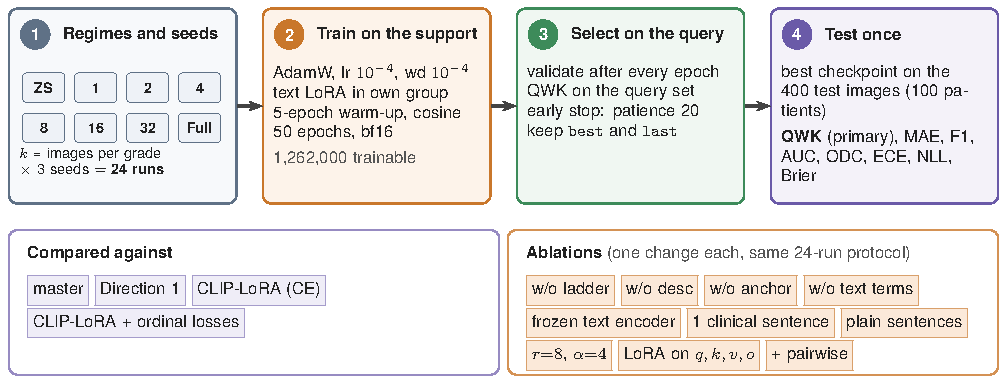
\includegraphics[width=\linewidth]{protocol_d2}
\caption{\lr{protocol} آزمایش‌های جهت ۲.}
\label{fig:proto-d2}
\end{figure}

\begin{figure}[H]
\begin{diagram}
  \node[train=4.4cm] (a) {Phase 1: Dir.~2 · 24 runs};
  \node[box=4.4cm,below=of a] (b) {Compare with master, Dir.~1 \& Dir.~3};
  \node[decision,below=of b] (c) {Dir.~2 is best?};
  \node[train=5cm,below=of c] (d) {Phase 2: CLIP-LoRA \& ordinal variant + 11 ablations};
  \node[lossn=5cm,below=of d] (e) {Diagnostics: ladder, desc.~spread, anchor distance};
  \draw[arr] (a)--(b); \draw[arr] (b)--(c); \draw[arr] (c)--node[elabel,right]{yes}(d); \draw[arr] (d)--(e);
\end{diagram}
\caption{گردش کار آزمایش‌های جهت ۲.}
\label{fig:d2-flow}
\end{figure}
